%\pagebreak
\chapter{Hubschrauber für Infanteristen}
\label{HuFIn}
\section{Hubschrauber}
	Helikopter können sehr vielseitig eingesetzt werden. Sie können Gebiete großflächig aufklären, Truppen und Güter transportieren, Personen in Not helfen und vieles mehr. Damit diese Einsätze so schnell und leicht wie möglich ohne viel Aufwand abgewickelt werden können, gibt es einige Hilfsmittel und Richtlinien. Nachfolgend werden die gängigsten Helikoptertypen im TTT näher erklärt. 
\subsection{Modellübersicht}
\paragraph*{UH-60 Blackhawk}
	\begin{itemize}
		\item 4 Mann Besatzung (2 Piloten, 2 Gunner); 12 Infanteristen 
		\item 2x 7,62mm Minigun 
		\item 168 Täuschkörper in Mehrfachwurf (24 Stück) oder automatisch (2 Stück pro 
		Sekunde, 8 Sekunden lang) 
	\end{itemize}
\paragraph*{CH-47 Chinook}
	\begin{itemize}
		\item 4 Mann Besatzung (2 Piloten, 2 Gunner); 24 Infanteristen 
		\item 2x 7,62mm Minigun 
		\item 168 Täuschkörper in Mehrfachwurf (24 Stück) oder automatisch (2 Stück pro 
		Sekunde, 8 Sekunden lang) 
	\end{itemize}

\section{Allgemein}
\subsection{Verhalten außerhalb}
	\begin{itemize}
		\item Bei Helikoptern mit seitlichem Aufstieg hat sich die Infanterie frontal dem  
		Hubschrauber zu nähern, um dann in einem Bogen seitlich aufzusteigen. Somit hat 
		die Besatzung jederzeit Blickkontakt.  
		\item Wenn man mit einem bewaffneten Luftfahrzeug operiert, ist jederzeit genug Abstand 
		zu den Waffensystemen zu halten LEBENSGEFAHR
		\item Bei Hanglage ist auf die Rotoren zu achten, da diese, bedingt durch die Schräglage  
		des Fahrzeuges, dem Boden äußerst nahe kommen und somit schwerste 
		Verletzungen anrichten können. 
		\item Immer gilt: Anweisungen der Crew sind Folge zu leisten! Das letzte Wort hat immer  
		der Pilot! 
	\end{itemize}
\subsection{Verhalten innerhalb}
	Die truppinternen Gespräche der Infanterie sollten sich im Helikopter auf ein Minimum reduzieren. Wenn Funkabsprachen unausweichlich sind, sollte die Lautstärke von TFAR auf “Whispern” eingestellt werden, sodass die Helikopterbesatzung ungestört ihrem Dienst nachkommen kann.\par
	Aufgabe der Infanterie im Flug ist es, nach allen Bedrohungen Ausschau zu halten beispielsweise Gewehrfeuer, Raketenbeschuss oder generelles Mündungsfeuer, Bewegungen von Feinden, Hindernissen oder jeglichen anderen Gefahren für das Fahrzeug. Hierbei sollte der Pilot immer umgehend über diese Bedrohungen informiert werden.

\section{Verlegung von Infanterie}
	Vor Einsatzbeginn sind folgende Fragestellungen zu klären:
	\par\medskip
	\begin{tabular}{ll}
	WO  & ist der geplante Landeraum?\\ 
	WAS  & wird transportiert?\\ 
	WIE  & wird verlegt?\\ 
	WER  & steigt auf?\\ 
	\end{tabular}
	\par\medskip
	Falls es keinen FAC gibt, welcher die Ressource über die OPL beantragt, wählt sich die Nr.2 auf die SR der Helikopterbesatzung ein, um später dem Piloten mitzuteilen, dass alle Teile seines jeweiligen Trupps erfolgreich abgesessen sind. Es wird immer vom Rang niedrigsten beginnend abgestiegen.\par
	Sobald der Pilot den “Touchdown” durchgibt, geht die Befehlsgewalt über die Infanterie wieder an den Truppführer über. Dieser kann nun das eigentliche absteigen befehlen.

\section{Ablaufplan von Extraktion, MedEvac oder Logistik}
\subsection{Anforderung der Ressource}
	Bedingt durch die Einbindung mehrerer Truppteile müssen angeforderte Ressourcen wie MedEvac, Logistik etc. vom Operationsleiter genehmigt werden. Hierzu setzt sich der Forward Air Controller (FAC) mit der OPL in Verbindung und beantragt die Ressource mit Begründung. Der Operationsleiter entscheidet anschließend situationsgerecht und gibt die Ressource entweder frei oder lehnt diese ab. Im Anschluss darauf findet der FAC sich wieder auf seinem eigenen Funkkreis ein, um von der jeweiligen Ressource direkt kontaktiert zu werden. 

\subsection{Landezone finden und einrichten}
	Der FAC verschafft sich in der Zwischenzeit im Einsatzgebiet einen kurzen Überblick über die Topographie und entscheidet im Anschluss darauf, an welcher Position sich im besten Falle die Landezone befindet. Gleichzeitig legt er auch eine sekundäre Landezone für den Notfall fest und markiert beide Positionen entsprechend mit gültiger Beschriftung auf der Karte (siehe hierzu “SGA FAC” von LingLing).\par
	Eine optimale LZ bietet sowohl für den Anflug des Helikopters, als auch für die Infanterie genügend Deckung. Im optimalen Fall sieht der Pilot die LZ schon von weitem bzw. wird frühzeitig über den FAC mittels Landmarke eingewiesen. Die LZ sollte möglichst eben und frei von Hindernissen sein, welche dem Helikopter schaden könnten. Hierbei muss die Größe so gewählt sein, dass genügend Raum für den Helikopter im Landeanflug sichergestellt ist. 
	\begin{figure}[htbp]
		\centering
		\includegraphics[width=0.95\linewidth]{../img/advanced/hubschrauber_+_infanterie/landezone}
	\end{figure}
	\begin{figure}[htbp]
		\centering
		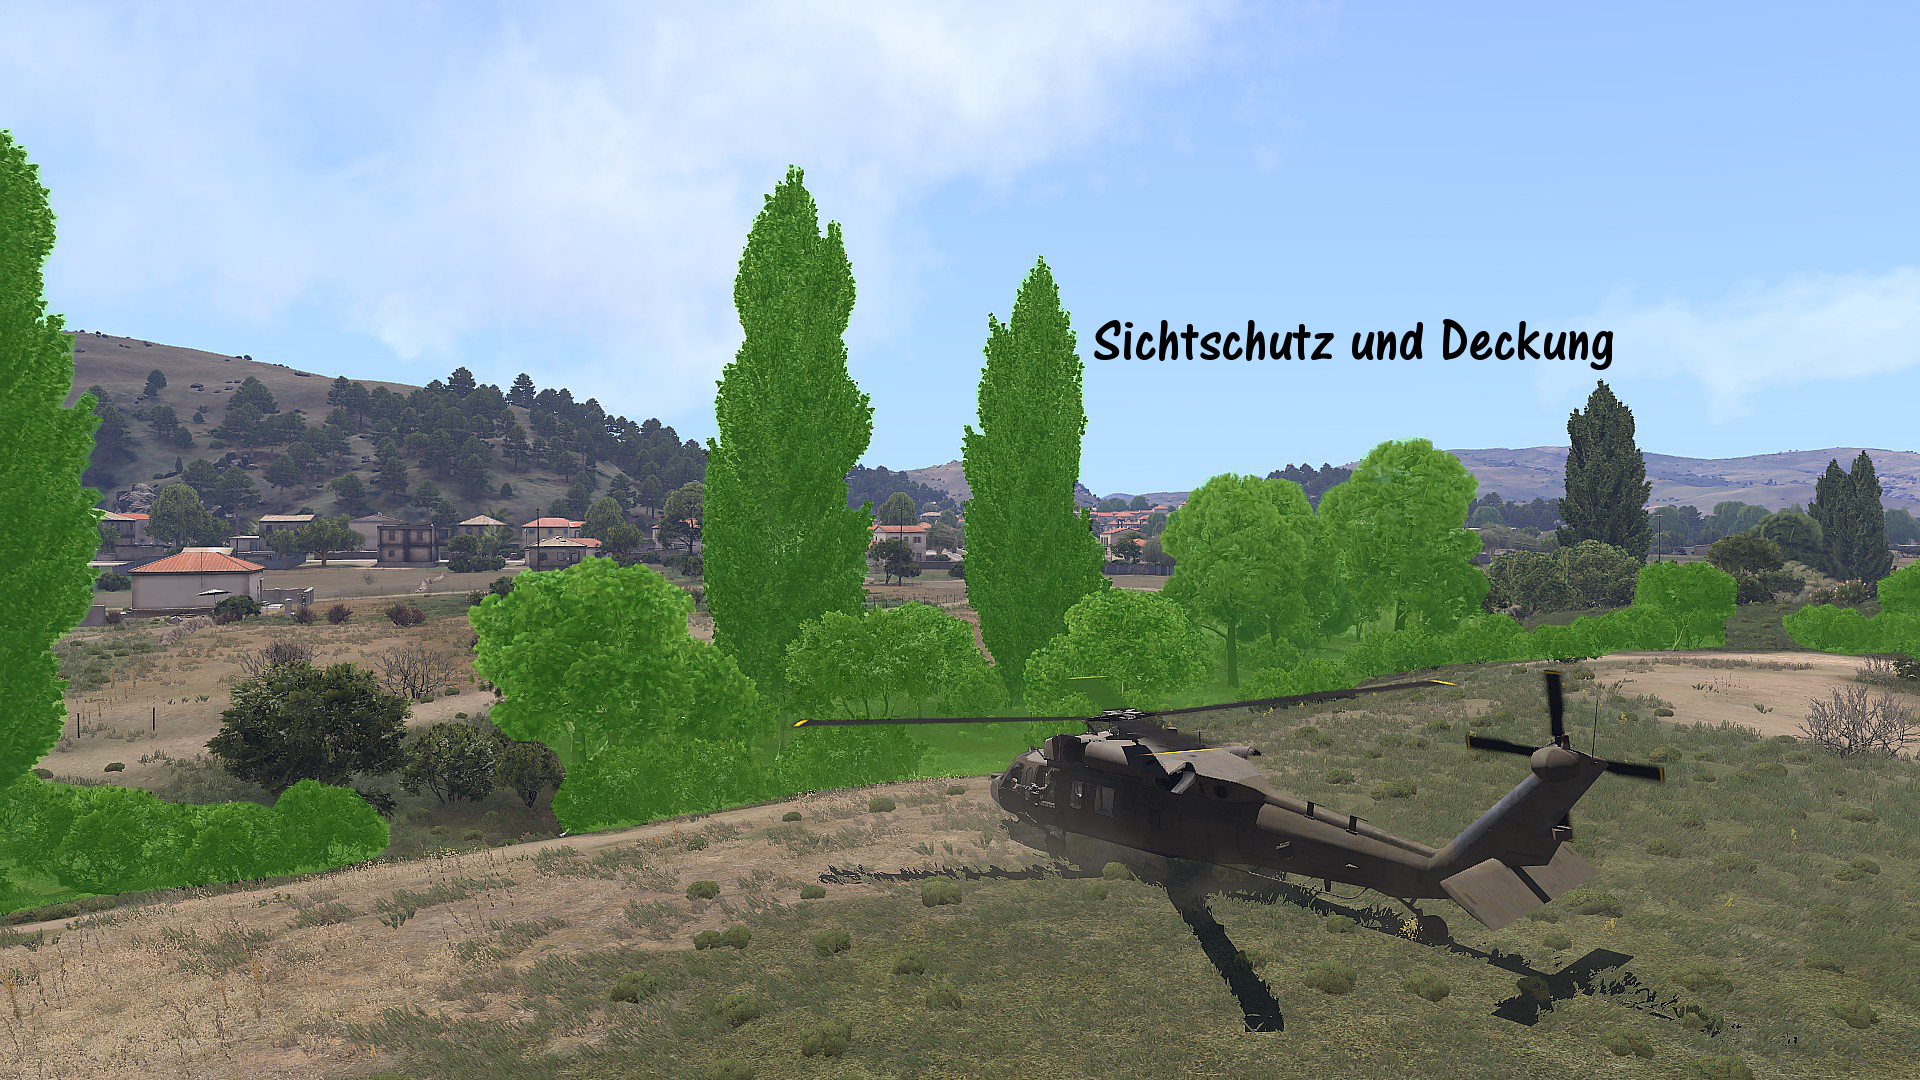
\includegraphics[width=0.95\linewidth]{../img/advanced/hubschrauber_+_infanterie/verdeckte-landung}
	\end{figure}	

\subsubsection{Heiße Landezonen}
	Bei heißen Landezonen kommt es auf eine gute Reaktion der Infanterie und vor allem Schnelligkeit an. Zur besseren Deckung können die Soldaten Rauchgranaten einsetzen, ebenso kann der Pilot das Einrauchen der Landezone befehlen, um die Sichtlinie zu eventuellen Feindkräften zu brechen.\par
	Wenn ein Helikopter eine bereits unter Beschuss stehende Landezone anfliegen soll, ist der Pilot im Voraus darüber zu unterrichten. Da der Pilot zu jedem Zeitpunkt die vollständige Verantwortung über das Luftfahrzeug inkl. Besatzung inne hat, kann dieser zu jedem Zeitpunkt den Anflug abbrechen oder die Landezone verlassen.\par
	Eine Besonderheit stellt das Aufsitzen der Infanterie unter Beschuss dar hierbei wird die normale Aufsitzreihenfolge missachtet, um ein schnelles Aufsitzen der gesamten Kräfte zu ermöglichen.

\subsection{Informationsfluss}
	Die Helikopterbesatzung wird seitens der OPL über die Anforderung der Ressource mit Angabe des Antragstellers informiert. Nach Bestätigung des Auftrags verbindet sich die Besatzung direkt mit dem jeweiligen Trupp und meldet Einsatzbereitschaft. Nun muss der FAC den im Voraus vorbereiteten 5-Liner an die Besatzung übermitteln. Nach erfolgreichem Readback setzt sich der Helikopter in Bewegung und hält ständigen Funkkontakt, um ggf. plötzliche Änderungen oder wichtige Hinweise durchzugeben oder seitens des FACs zu erhalten.
	\par\medskip
	In Sonderfällen kann der FAC die Ressource zunächst in eine Holding Postition beauftragen und im Anschluss, je nach Situationslage, den 5-Liner an die Besatzung übermitteln oder den Einsatz komplett abbrechen.
	\par\medskip 
	Anmerkung: Falls die Verbindung zwischen Helikopter und FAC ausfallen sollte, wählt sich der Pilot selbstständig sofort auf dem SR Kanal des Trupps ein, um eine Funkverbindung wiederherzustellen.

\subsection{Landeanflug - Die Einweisung/ die Übergabe an den Einweiser}
	Der Pilot meldet die Annäherung an den Operationsraum. In diesem Moment geht die komplette Verantwortung zum FAC über. Er befiehlt dem FAC das markieren der Landezone durch Leucht oder Rauchmarkierungen. Der FAC weist auf Anforderung den Piloten in die korrekte Position ein und warnt ihn ggf. über Gefahren.\par
	Tipp: Bei Nacht sieht man sehr gut ein Knicklicht in Kombination mit einer Rauchgranate, welche darauf geschmissen wird.
	\par\medskip
	Sobald der Pilot den “Touchdown” durchgibt darf die Infanterie die nötigen Aufgaben durchführen.\par
	Warum man einen FAC braucht, hier in einem Video verdeutlicht:\\
	\url{https://www.youtube.com/watch?v=NJIZTL2ZyEw}

	\begin{figure}[htbp]
		\centering
		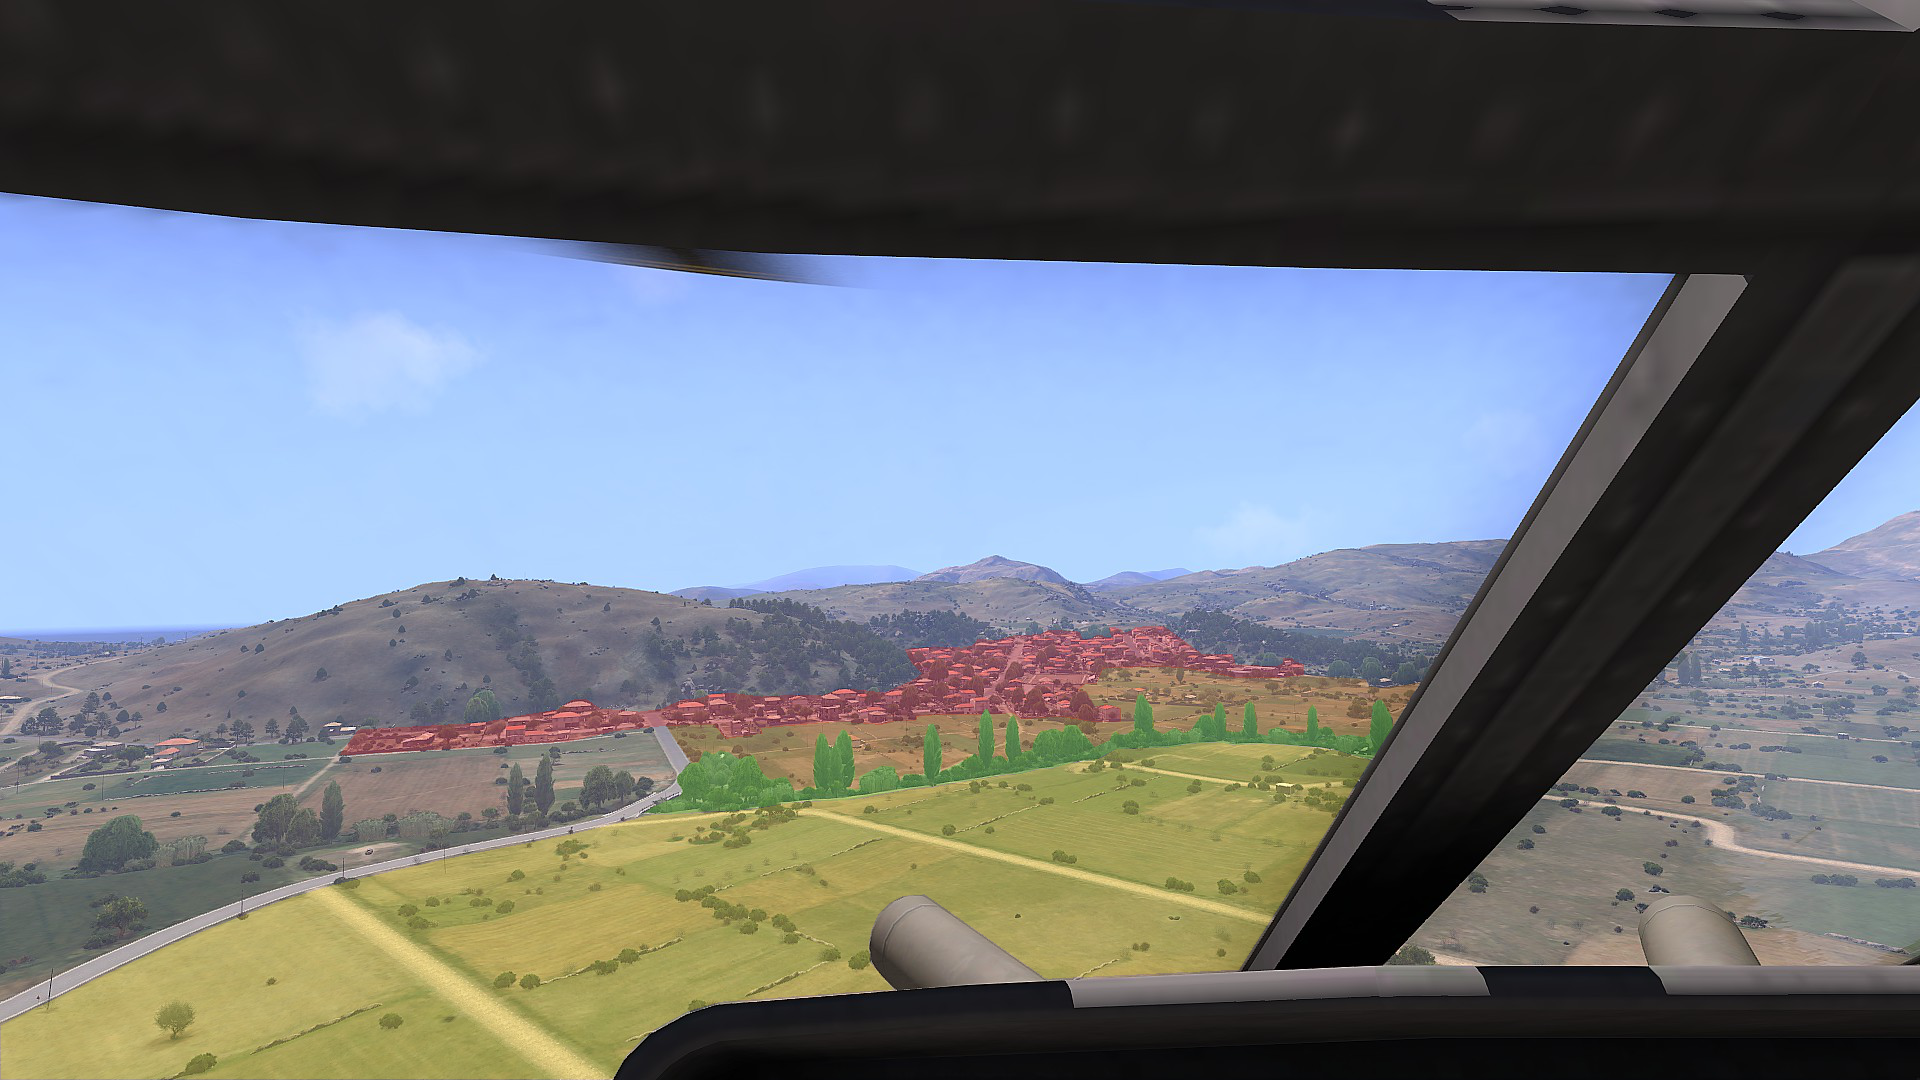
\includegraphics[width=0.95\linewidth]{../img/advanced/hubschrauber_+_infanterie/sicht-pilot}
	\end{figure}

\subsection{Lift-off}
	Sobald alle Aufgaben abgeschlossen sind oder der FAC die vollständige Anwesenheit durchgibt, führt der Pilot den Lift-off durch. In diesem Moment erlischt die Verantwortung vom FAC. 

\subsection{Worst Case Szenarios}
	Falls während dem Flug die Maschine beschädigt wird, werden alle Pläne und Aufträge verworfen. In diesem Moment ist oberste Priorität die Maschine unversehrt zu landen. In dem Fall, dass ein Helikopter bei einer Landung beschädigt wird, sind die nötigen Maßnahmen zu veranlassen den Helikopter wieder Instand zu setzen.